%%%%%%%%%%%%%%%%%%%%%%%%%%%%%%%%%%%%%%%%%%%%%%
%                insertmeeting
% 1) Title (something creative & funny?)
% 2) Date (MM/DD/YYYY)
% 3) Location (ex. Hagerty High School)
% 4) People/Committees Present 
% 5) Picture 
% 6) Start Time & Stop Time (ex. 12:30AM to 4:30PM)
%%%%%%%%%%%%%%%%%%%%%%%%%%%%%%%%%%%%%%%%%%%%%%
\insertmeeting 
	{The Power of 3D Printing} 
	{10/16/21}
	{Hagerty High School}
	{Nathan, Ritam, Samantha}
	{Images/RobotPics/robot.jpg}
	{11:00 - 12:30}
	
\hhscommittee{Hardware}
\noindent\hfil\rule{\textwidth}{.4pt}\hfil
\subsubsection*{Goals}
\begin{itemize}
    \item Start printing drivetrain  

\end{itemize} 

\noindent\hfil\rule{\textwidth}{.4pt}\hfil

\subsubsection*{Accomplishments}
It’s finally time to print the drivetrain! After spending hours designing this drivetrain, we were almost ready to start printing, but before we could start up the 3d printer, we needed to ensure the design looked right in CAD. One thing we noticed was that the cutouts for the pulleys or sprockets were too small. Although big enough for the pulleys and sprockets themselves, when we connect a belt or chain, the chain will hit the edge of the plastic. Because of this , we expanded the hole to allow the belt or chain to fit through (Figure \ref{fig:101621_1}). We then continued to adjust several smaller features like changing the fillets on the ribs, and changing the tolerance on the holes. With hopefully everything in order, we put the parts into a slicer and sent them to the fortus 450 printer. The whole drivetrain will be solid polycarbonate, a very strong plastic that should survive all of the bumps and crashes that it might take during the competition. Because the print is going to take 12 hours, we are waiting patiently but excitedly to see the final product.


\begin{figure}[htp]
\centering
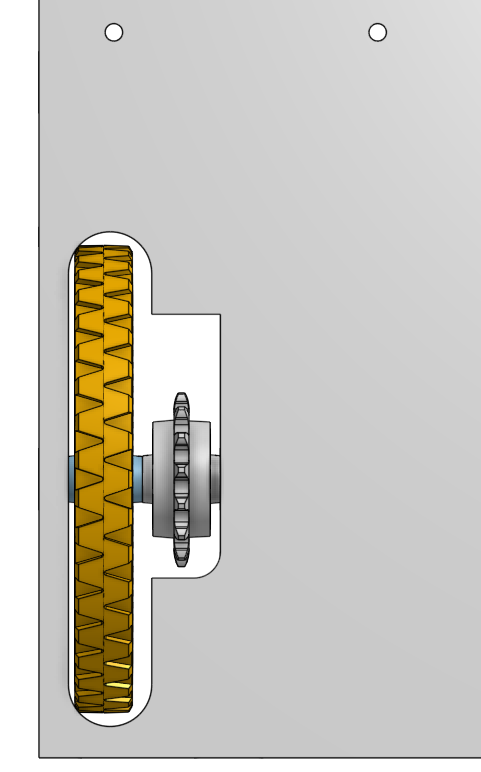
\includegraphics[width=0.95\textwidth, angle=0]{Meetings/October/10-16-21/10-16-21_Hardware_Figure2 - Nathan Forrer.PNG}
\caption{Our solution to the incorrect CAD.}
\label{fig:101621_1}
\end{figure}

\whatsnext{
\begin{itemize}
    \item Assemble drivetrain
\end{itemize} 
}

